\documentclass[crop,tikz]{standalone}% 'crop' is the default for v1.0, before it was 'preview'
%\usetikzlibrary{...}% tikz package already loaded by 'tikz' option
\usepackage{graphicx}
\usepackage{amsmath}
\usepackage{amsfonts}
\usepackage{amssymb}
\usepackage{amsthm}
\usepackage{bbold}
\usepackage[nomessages]{fp}

\usetikzlibrary{arrows,calc,decorations.pathmorphing,backgrounds,positioning,fit,intersections}
\usetikzlibrary{automata,shapes}


\usetikzlibrary{arrows,calc,positioning}
\tikzset{>=angle 60}

% colors
\newcommand{\tcR}[1]{\textcolor{red!60!black}{#1}}
\newcommand{\tcRR}[1]{\textcolor{red}{#1}}
\newcommand{\tcG}[1]{\textcolor{green!60!black}{#1}}
\newcommand{\tcB}[1]{\textcolor{blue!60!black}{#1}}
\newcommand{\tcO}[1]{\textcolor{orange!90!black}{#1}}
\newcommand{\tcP}[1]{\textcolor{blue!50!red!90!black}{#1}}

\begin{document}
{\scriptsize
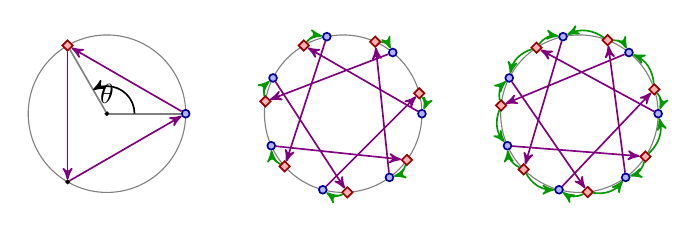
\begin{tikzpicture}[
        scale=0.5, ->, 
        >=stealth', 
        auto, 
        point/.style = {draw=blue!60!black, circle,  fill = blue!30!white, inner sep = 1.0pt},
        imgpoint/.style = {draw=red!60!black, diamond,  fill = red!30!white, inner sep = 1.0pt},
        dot/.style = {draw, circle,  fill = black, inner sep = 0.1pt},
        rho/.style = {blue!50!red!100!black},
        pi/.style = {green!60!black},
        semithick]
    
    \def\rad{2}
    \def\hshift{6}
    
    \draw[gray,thin] (0,0) circle (\rad); 
    \node (0) at +(0:0) [dot] {};
    \node (1) at +(0:\rad) [point] {};
    \node (2) at +(120:\rad) [imgpoint] {};
    \node (3) at +(240:\rad) [dot] {};
    \path (1) edge [rho] (2)
        (2) edge [rho] (3)
        (3) edge [rho] (1);
    \draw[gray,-] (0) -- (2);      
    \draw[gray,-] (0) -- (1); 
    \draw (0,0) +(0:0.7) arc (0:120:.7);  
    \node [above] at (0) {$\theta$};   

\begin{scope}[shift={(\hshift,0)}]     
    
    \draw[gray,thin] (0,0) circle (\rad); 
	\foreach \i in {0,...,6}
		{
    		\node[point] (\i) at (\i*51:\rad) {};
	   		\node[imgpoint] (\i+7) at (\i*51+120:\rad) {};
		}
	\path (0) edge [rho] (0+7);
	\path (0+7) edge [pi, bend left] (2);
	\path (1) edge [rho] (1+7);
	\path (1+7) edge [pi, bend left] (3);
	\path (2) edge [rho] (2+7);
	\path (2+7) edge [pi, bend left] (4);
	\path (3) edge [rho] (3+7);
	\path (3+7) edge [pi, bend left] (5);
	\path (4) edge [rho] (4+7);
	\path (4+7) edge [pi, bend left] (6);
	\path (5) edge [rho] (5+7);
	\path (5+7) edge [pi, bend left] (0);
	\path (6) edge [rho] (6+7);
	\path (6+7) edge [pi, bend left] (1);


\begin{scope}[shift={(\hshift,0)}]     

    \draw[gray,thin] (0,0) circle (\rad); 
	\foreach \i in {0,...,6}
		{
    		\node[point] (\i) at (\i*51:\rad) {};
	   		\node[imgpoint] (\i+7) at (\i*51+123:\rad) {};
		}

	\path (0) edge [rho] (0+7);
	\path (1) edge [rho] (1+7);
	\path (2) edge [rho] (2+7);
	\path (3) edge [rho] (3+7);
	\path (4) edge [rho] (4+7);
	\path (5) edge [rho] (5+7);
	\path (6) edge [rho] (6+7);

	\path (0+7) edge [pi, bend left] (2);
	\path (0+7) edge [pi, bend right] (3);
	\path (1+7) edge [pi, bend left] (3);
	\path (1+7) edge [pi, bend right] (4);
	\path (2+7) edge [pi, bend left] (4);
	\path (2+7) edge [pi, bend right] (5);
	\path (3+7) edge [pi, bend left] (5);
	\path (3+7) edge [pi, bend right] (6);
	\path (4+7) edge [pi, bend left] (6);
	\path (4+7) edge [pi, bend right] (0);
	\path (5+7) edge [pi, bend left] (0);
	\path (5+7) edge [pi, bend right] (1);
	\path (6+7) edge [pi, bend left] (1);
	\path (6+7) edge [pi, bend right] (2);
\end{scope}    
\end{scope}    

\end{tikzpicture}
}
\end{document}
